\chapter{REQUIREMENTS AND SPECIFICATION}
\label{chap:requirements}

% GradeCalc aims to be the first choice of students. To be in that precious spot, it will have to fit the student's needs perfectly. The following ones are the requirements I collected from asking colleagues and filtering brainstormed ideas.

This section defines and explains the requirements of the application. They are obtained by analyzing how students manage their grades and coming up with solutions that would help them be more productive. They are also obtained by directly asking what potential users would want in the app.

\section{Functional requirements}
\label{sec:user-stories}

This section presents the requirements of the app in the form of user stories (US).

% \begin{titlebox}{TODO}
%   Use some sort of table and for each requirement set: id, title, description, acceptation criteria
% \end{titlebox}

% \begin{titlebox}{TODO}
%   Add acceptation criteria
% \end{titlebox}

% Criteris d'acceptacio son molt importants, posar un google forms inventat

% no cal model de comportament

\nextUserStory{Calculate needed grade}\label{us:x}
\usStatement{user}{calculate needed grade to pass a course}{decide how much to study}

\nextUserStory{Calculate final grade}\label{us:x}
\usStatement{user}{calculate my final grade assuming a 0 in the remaining exams}{know if I already passed}

\nextUserStory{Current grades}\label{us:x}
\usStatement{user}{see my current grades}{view my performance}

\nextUserStory{Sign-up}\label{us:x}
\usStatement{user}{sign-up with an external authentication provider}{register faster and more conveniently.}

\nextUserStory{Log-in and Log-out}\label{us:x}
\usStatement{user}{log-in and Log-out}{decide when to use my account}

\nextUserStory{Save grades in my account}\label{us:x}
\usStatement{user}{save grades in my account}{share them between my desktop and mobile}

\nextUserStory{Save grades in the device}\label{us:x}
\usStatement{user}{save grades in the device}{use the app without an account or offline}

\nextUserStory{Create subject}\label{us:x}
\usStatement{user}{create subject}{use the app with any of my courses}

\nextUserStory{Edit subject}\label{us:x}
\usStatement{user}{edit subject}{correct mistakes or tweak values}

\nextUserStory{View subject}\label{us:x}
\usStatement{user}{view subject details}{see clearly all it's information}

\nextUserStory{Delete subject}\label{us:x}
\usStatement{user}{delete subject}{focus on other subjects}

\nextUserStory{Search subjects}\label{us:x}
\usStatement{user}{search subjects}{avoid creating them and save time}
% typos
% instant

\nextUserStory{Multiple evaluations}\label{us:x}
\usStatement{user}{be able to set have multiple evaluation formulas on subjects}{represent my subject's evaluation precisely}
% can share exams
% can have unique exams

% \nextUserStory{Subjects can have optional exams}\label{us:x}
% \usStatement{user}{subjects can have optional exams}{}

% \nextUserStory{Subjects' evaluations can share exams}\label{us:x}
% \usStatement{user}{subjects' evaluations can share exams}{}

\nextUserStory{Dashboard}\label{us:x}
\usStatement{user}{have a dashboard with my subjects}{handily input my grades}

% \nextUserStory{Quick view of my current grades (subject bar)}\label{us:x}
% \usStatement{user}{quick view of my current grades (subject bar)}{}

\nextUserStory{Auto-evaluate}\label{us:x}
\usStatement{user}{automatically reevaluate the calculations}{see the right values all the time}

\nextUserStory{Auto-save}\label{us:x}
\usStatement{user}{automatically save my changes}{save time saving and don't forget to save}

\nextUserStory{Auto-sync}\label{us:x}
\usStatement{user}{automatically syncs my changes with my account}{have a consistent state always}

\nextUserStory{Responsive UI}\label{us:x}
\usStatement{user}{have UI designed for mobile and desktop}{use the app in any screen size}

\nextUserStory{Use from browser}\label{us:x}
\usStatement{user}{use the app from the browser}{use it without downloading it}

\nextUserStory{Lunch icon}\label{us:x}
\usStatement{user}{have a lunch icon on the home screen}{quickly open the app}
% install from browser
% install from play store

% \nextUserStory{Install from browser}\label{us:x}
% \usStatement{user}{install the app from the browser}{quickly open the app}

% \nextUserStory{Download from Play Store}\label{us:x}
% \usStatement{user}{download the app from the Google Play Store}{download it like any other app}

\nextUserStory{Offline}\label{us:x}
\usStatement{user}{use the app offline}{use it without depending on my internet connection}

\nextUserStory{SEO}\label{us:x}
\usStatement{user}{find the app in Google}{open it without knowing the domain}

\nextUserStory{Tutorial}\label{us:x}
\usStatement{user}{have a tutorial}{learn to use the app the first time I visit it}

\nextUserStory{Undo}\label{us:x}
\usStatement{user}{be able to undo some actions}{fix mistakes}

\nextUserStory{Notifications}\label{us:x}
\usStatement{user}{be notified with tips and suggestions inside the app}{take advantage the app,  and use it correctly}

\nextUserStory{Accessible}\label{us:x}
\usStatement{user}{still be able to use the app if I have a disability}{use the app without complications}

\nextUserStory{Updates}\label{us:x}
\usStatement{user}{receive frequent updates}{enjoy the latest features}
% this sets CD

\nextUserStory{Analytics}\label{us:x}
\usStatement{user}{give data of my usage up (anonymized)}{improve the app}

% \nextUserStory{Implement Continuous Integration and Deployment}\label{us:x}
% \usStatement{user}{implement Continuous Integration and Deployment}{}

\nextUserStory{Open-source}\label{us:x}
\usStatement{user}{have the main code publicly available (open-source)}{validate that the app does what it states}

\nextUserStory{Background activity}\label{us:x}
\usStatement{user}{be aware of background activity}{better predict the behavior of the app}

\nextUserStory{In Spanish}\label{us:x}
\usStatement{user}{have the app entirely in Spanish}{understand it}

\nextUserStory{Legal page}\label{us:x}
\usStatement{user}{have a page with legal information}{solve any doubts}


% \nextUserStory{Create subject}\label{us:create-subject}
% \usStatement{user}{create a subject}{use it}
% US\ref{us:create-subject}



\clearpage\newpage
\section{Non-Functional requirements}
\label{sec:non-functional}

% \subsection{For the students}
% \begin{multicols}{3}
% \noindent
% Be \textbf{reliable}:
% \vspace{-5mm}
% \begin{itemize}[leftmargin=*]
%     \setlength\itemsep{-1em}
%     \item Don't lose data.
%     \item Don't miscalculate.
%     \item Keep grades private.
%     \item Work as expected.
%     \item Work on all devices.
%     \item Work offline.
% \end{itemize}
% \columnbreak
% \noindent
% Be \textbf{easy to learn} and use:
% \vspace{-5mm}
% \begin{itemize}[leftmargin=*]
%     \setlength\itemsep{-1em}
%     \item Simple and attractive UI.
%     \item Feel fast.
%     \item Place elements where expected.
%     \item Shows clearly where results come from.
% \end{itemize}
% \columnbreak
% \noindent
% Be \textbf{engaging}:
% \vspace{-5mm}
% \begin{itemize}[leftmargin=*]
%     \setlength\itemsep{-1em}
%     \item Get updates.
%     \item Have "cool" details.
%     \item Encourage to share the app.
%     \item Have an easy to remember name, logo, and domain.
% \end{itemize}

% \end{multicols}

% \subsection{For the developers}

% \begin{itemize}
%     \setlength\itemsep{-1em}
%     \item Have the minimum economic costs, zero if possible.
%     \item Use modern technologies.
%     \item Generate some economic income to pay for expenses.
%     \item Use open source technologies.
% \end{itemize}

This section highlights the 4 non-functional requirements (NFR) that the application must meet. These requirements shape the app so much that all features aim to satisfy them.

\subsection*{NFR 1 - Reliable}
\begin{itemize}
    \item \textbf{Description}: The functionalities have to work consistently and predictably, in other words, the app has to work as the user expects. For example, it doesn't lose data, it doesn't miscalculate, it works on all the user's devices, it works offline...
    \item \textbf{Justification}: The app has to work properly to be useful, otherwise there's no point in using it.
    \item \textbf{Acceptance criteria}: Ask a sample of users to evaluate, from 1 to 5, how much they agree to the following statements. A mean greater than 2.5 needs to be achieved.
    \begin{itemize}[noitemsep]
        \item The app works as I expect.
        \item The app does the calculations without mistakes.
        \item I can use the app from any of my devices.
        \item The app has never lost any of my data.
        \item I can use the app with the subjects I course.
    \end{itemize}
\end{itemize}

\subsection*{NFR 2 - Easy to use}
\begin{itemize}
    \item \textbf{Description}: The app has to be intuitive and accessible, in other words, easy to learn and easy to use.
    \item \textbf{Justification}: If the app is easy to use the users will save time and overall be more satisfied.
    \item \textbf{Acceptance criteria}: Ask a sample of users to evaluate, from 1 to 5, how much they agree to the following statements. A mean greater than 2.5 needs to be achieved.
    \begin{itemize}[noitemsep]
        \item The app is easy to learn
        \item The app is easy to use
        \item The app responds quickly to my actions.
        \item I know how to use the app in general.
        \item I know how to create a subject
        \item I understand all the information in the dashboard.
    \end{itemize}
\end{itemize}

\subsection*{NFR 3 - Engaging}
\begin{itemize}
    \item \textbf{Description}: The app must engage users and ensure that they are enjoying it and will recommend it.
    \item \textbf{Justification}: Happy users will attract new users helping the app grow. If the users are engaged, that means that the app is useful to them.
    \item \textbf{Acceptance criteria}: Ask a sample of users to evaluate, from 1 to 5, how much they agree to the following statements. A mean greater than 2.5 needs to be achieved.
    \begin{itemize}[noitemsep]
        \item I enjoy using the app.
        \item I would recommend the app.
        \item There's people using the app thanks to me.
        \item The app helps me to achieve my goals.
        \item The app helps me to pass the subjects.
        \item I open the app frequently.
        \item I open the app when I receive a new grade.
        \item GradeCalc's logo, name, and style are easy to remember.
        \item I like GradeCalc's logo, name, and style.
    \end{itemize}    
\end{itemize}

\subsection*{NFR 4 - Cheap to produce}
\begin{itemize}
    \item \textbf{Description}: The app has to be as cheap as possible to develop and maintain.
    \item \textbf{Justification}: This is a small hobby project developed by a student that is not willing to spend money on it unless it's imperceptible or would make a big difference.
    \item \textbf{Acceptance criteria}: the app must have a profit greater than -50€/year and cost less than 100€ to develop.
\end{itemize}


\section{Conceptual model}

The app has two main entities, subjects, and students, they are marked with thicker borders. 
\begin{itemize}
    \item Students are the users of the app and they can create and course subjects.
    \item Subjects are what students course that lead to an examination or qualification. A subject is taught in a faculty, and a faculty belongs to a university. Also, subjects are done in a course (usually a semester). 
    \item Faculty, university, and course are not relevant for the app's requirements, they are just related concepts, so in the database, they'll be just attributes of a subject, not standalone classes.
    \item A subject contains one or more evaluations and one or more exams. An evaluation contains exams with weights.
\end{itemize}

The main takeaway from the conceptual model (Fig. \ref{fig:conceptual-model}) is that students create and course subjects, and subjects have evaluations with exams and basic information to be searched like short name, full name, university or course. 

\vfill
\begin{figure}[ht!]
    \center
    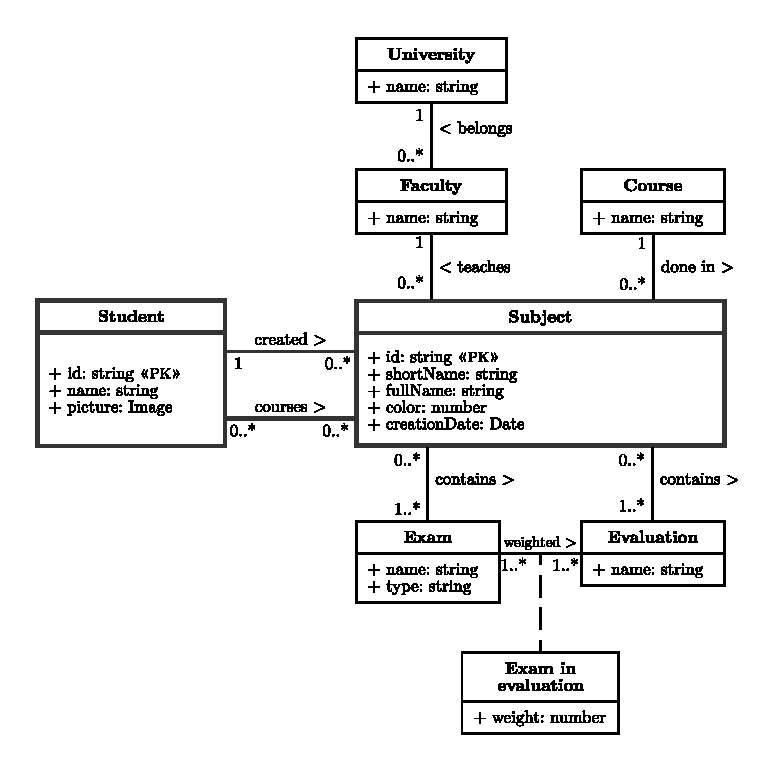
\includegraphics[width=\linewidth]{media/diagrams/conceptual.pdf}
    \caption{Conceptual model's UML Diagram}
    \label{fig:conceptual-model}
\end{figure}
\vfill

\clearpage\newpage
\section{Tasks}

This section defines all the tasks to do in order to fulfill all the requirements that the application must meet. These tasks are very specific and can be directly placed into the Kanban board. They are organized by screens and components of the app. This section will help understand all the features implemented and it's level of detail.

% This section defines all the functional requirements that the application must meet.
% Overall, the app may look like it does a few things, but the ones it does are very polished. For example, the subject card alone has a tone of features, and looking at it in a glance seems that it must be trivial, but it has many small details that make the app truly productive and enjoyable. To come up with these requisites, there was an intense thought process to find the simplest way to present the features to the user.


\subsection*{Dashboard}
A user wants to see and interact with his subjects and grades.

\begin{itemize}[leftmargin=2cm]
    \item[\nextTask{}\label{req:x}] It is the homescreen of the app.
    \item[\nextTask{}\label{req:x}] It contains subject cards.
    \item[\nextTask{}\label{req:x}] When the app is opened, the subjects are retrieved from the device's local storage. And a non blocking spinner is shown while the subjects are being loaded.
    \item[\nextTask{}\label{req:x}]  When the app is opened and the user is logged-in, subjects are synced with his account. While this happens a non blocking spinner appears.
    \item[\nextTask{}\label{req:x}] The subject cards are sorted alphabetically by \textit{shortName}.
    \item[\nextTask{}\label{req:x}] When there are no subject cards, the add button starts a looping animation, similar to the rubberBand from the Animate.css\cite{animate-css} library, to draw attention.
    \item[\nextTask{}\label{req:x}] When there are no subject cards, the empty space is replaced with an explanatory text about the app. At the end of the text, there are instructions to add the first subject. This text serves two purposes, inform the user, and optimize the search engine indexing of the app.
    \item[\nextTask{}\label{req:x}] It has a header bar on top of the subject cards and in the top of the screen.
    \begin{itemize}[leftmargin=2cm]
        \item[\nextTask{}\label{req:x}] The header bar has, in the left, an icon that when clicked goes to the login screen.
        \item[\nextTask{}\label{req:x}] The header bar has, in the center, the app name.
        \item[\nextTask{}\label{req:x}] The header bar has, in the right, an icon that when clicked goes to the search subject screen.
    \end{itemize}
    \item[\nextTask{}\label{req:x}] It is responsive and the subjects are rearranged depending on the screen width.
    \item[\nextTask{}\label{req:x}] When all subject cards displayed are passed, a present appears at the bottom of the dashboard along with a congratulating text.
    \item[\nextTask{}\label{req:x}] When the gift is clicked a funny congratulating video appears at the bottom of the screen and plays automatically in a loop.
    \item[\nextTask{}\label{req:x}] If the app meets the PWA installation criteria\cite{pwa-install-criteria}, a notification shows up with the install action.
\end{itemize}

\subsection*{Subject card}
A user wants to work with a specific subject in the dashboard.

\begin{itemize}[leftmargin=2cm]
    \item[\nextTask{}\label{req:x}] It can be in collapsed or expanded state.
    \begin{itemize}[leftmargin=2cm]
        \item[\nextTask{}\label{req:x}] A subject card is collapsed by default.
        \item[\nextTask{}\label{req:x}] When a subject card is expanded it pushes the other ones instead of overlapping them.
        \item[\nextTask{}\label{req:x}] When a subject card is clicked where there's no intractable elements, it toggles its state from collapsed or expanded. The intractable elements are the subject bar, exam input, evaluation selector, edit icon and delete button.
        \item[\nextTask{}\label{req:x}] There's an animation for when a subject card is collapsed or expanded.
        \item[\nextTask{}\label{req:x}] A collapsed card doesn't show the exams' inputs nor the evaluation selector. And a expanded one does. 
    \end{itemize}
    \item[\nextTask{}\label{req:x}] It has a graphical representation of the selected evaluation, called \textit{subject bar}. The representation is a bar divided in sections where each section represents an exam and it's length is proportional to the exam weight.
    \begin{itemize}[leftmargin=2cm]
        \item[\nextTask{}\label{req:x}] In the subject bar, hovering a section shows a tooltip displaying the exam weight in percentage.
        \item[\nextTask{}\label{req:x}] In the subject bar, each section contains the exam name and the grade. If the exam is undone, it contains the necessary grade instead.
        \item[\nextTask{}\label{req:x}] In the subject bar, the done exams have the subject's color as background color.
        \item[\nextTask{}\label{req:x}] In the subject bar, the undone exams have a light background color.
        \item[\nextTask{}\label{req:x}] In the subject bar, the exams are sorted by same order that they are in the exam array of the evaluation. Not alphabetically nor per weight.
        \item[\nextTask{}\label{req:x}] In the subject bar, when a section is clicked it focuses the exam's input. If the card is collapsed it's also expanded.
        \item[\nextTask{}\label{req:x}] In the subject bar, when a section is to narrow to see the full grade or name, the first characters are visible. Instead of the characters in the middle. 
    \end{itemize}
    \item[\nextTask{}\label{req:x}] It has the final grade in big text.
    \begin{itemize}[leftmargin=2cm]
        \item[\nextTask{}\label{req:x}] The final grade is calculated by multiplying each exam grade by its weight and summing all the values. If an exam is undone a 0 is used in the calculation.
        \item[\nextTask{}\label{req:x}] The final grade is green if it's greater or equal than five and red otherwise.
        \item[\nextTask{}\label{req:x}] The final grade is rounded to two decimals.
        \item[\nextTask{}\label{req:x}] When the final grade passes from a number lower than five to one greater or equal to five a confetti animation is triggered. The animation shoots confetti over the subject card to congratulate the user. 
    \end{itemize}
    \item[\nextTask{}\label{req:x}] It has an evaluation selector if there are more than one.
    \begin{itemize}[leftmargin=2cm]
        \item[\nextTask{}\label{req:x}] When the evaluation is changed, the card updates instantly it's information (exam inputs, subject bar, final grade...).
        \item[\nextTask{}\label{req:x}] If an exam with the same name is in more than one evaluations, the grade is shared among them. It means that the same exam can be used in different evaluations.
        \item[\nextTask{}\label{req:x}] The application remembers what is the selected evaluation. If the user closes and opens the app again, the selected evaluation doesn't change.
    \end{itemize}
    \item[\nextTask{}\label{req:x}] It has the subject's \textit{shortName} in big text.
    \item[\nextTask{}\label{req:x}] It has an input field for each exam in the selected evaluation.
    \begin{itemize}[leftmargin=2cm]
        \item[\nextTask{}\label{req:x}] The inputs are grouped by their type attribute.
        \begin{itemize}[leftmargin=2cm]
            \item[\nextTask{}\label{req:x}] The type is styled like a subtitle.
            \item[\nextTask{}\label{req:x}] Next to the type, there's the sum of the weights of the exams with that type in percentage and rounded.
            \item[\nextTask{}\label{req:x}] The types are sorted by the same order that they are in the exam array of the evaluation. Not alphabetically nor per weight.
            \item[\nextTask{}\label{req:x}] The exam inputs inside the type are sorted by same order that they are in the exam array of the evaluation. Not alphabetically nor per weight.
        \end{itemize}
        \item[\nextTask{}\label{req:x}] The exam input has different styles depending on it's vaule.
        \begin{itemize}[leftmargin=2cm]
            \item[\nextTask{}\label{req:x}] When the exam input has a valid value, it's considered a \textit{done exam}. It has the subject's color as background.
            \item[\nextTask{}\label{req:x}] When the exam input has an empty value, it's considered an \textit{undone exam}. It has a gray background and it's placeholder is the necessary grade to pass.
            \item[\nextTask{}\label{req:x}] When the exam input is focused it has a black border.
            \item[\nextTask{}\label{req:x}] When the exam input's value isn't a number nor empty, it has a gray background with red borders. And it's considered an \textit{undone exam}.
            \item[\nextTask{}\label{req:x}] When the exam input's value is a number but lower than 0 or greater than 10, it has the subject's color as background with red borders. And it's considered a \textit{done exam}.
            \item[\nextTask{}\label{req:x}] If the exam has weight 0, it's hidden.
        \end{itemize}
        \item[\nextTask{}\label{req:x}] At the left of the input there's a label with it's name.
        \item[\nextTask{}\label{req:x}] The exam input only accepts numbers (digits, periods, commas, plus, minus and e for exponential). And in digital keyboards shows a numeric keyboard.
        \item[\nextTask{}\label{req:x}] The necessary grade is the necessary grade to receive in all the remaining undone exams to get a 5 in the final grade.
        \item[\nextTask{}\label{req:x}] Every time a grade is changed other information is updated instantly.
        \begin{itemize}[leftmargin=2cm]
            \item[\nextTask{}\label{req:x}] The necessary grade is updated.
            \item[\nextTask{}\label{req:x}] The final grade is updated.
            \item[\nextTask{}\label{req:x}] If the user is logged-in, the new grade is sent to his account.
        \end{itemize}
        \item[\nextTask{}\label{req:x}] The exam inputs take a reasonable space for their expected value length, usually less than 6 characters.
        % \item[\nextTask{}\label{req:x}] The exam inputs can have 10 characters at maximum.
    \end{itemize}
    \item[\nextTask{}\label{req:x}] It has a edit icon.
    \begin{itemize}[leftmargin=2cm]
        \item[\nextTask{}\label{req:x}] The edit icon has a hover animation.
        \item[\nextTask{}\label{req:x}] When clicked opens the edit subject screen of the current subject. With the title ``Edit subject'' and the action button ``Save''.
        \item[\nextTask{}\label{req:x}] If the user finally edits the subject, the subject card's information is updated instantly (name, color, exam inputs...).
        \item[\nextTask{}\label{req:x}] If the user finally edits the subject, and he's logged-in, the subject is also edited in his account.
    \end{itemize}
    \item[\nextTask{}\label{req:x}] It has a delete button.
    \begin{itemize}[leftmargin=2cm]
        \item[\nextTask{}\label{req:x}] Hovering the card displays the delete button.
        \item[\nextTask{}\label{req:x}] The delete button has tree animations. On show it fades in and scales up to normal. On hover it shakes. On click it scales down.
        \item[\nextTask{}\label{req:x}] When the delete button is clicked the card is deleted.
        \item[\nextTask{}\label{req:x}] When a card is deleted, the other cards move to their new locations and sizes in a smooth animation.
        \item[\nextTask{}\label{req:x}] When a card is deleted, a notification appears saying "You deleted \textit{subject's shortName}"\space and a action button says "undo". When the action is clicked the subject is restored, like nothing happened. If the user is logged-in, undoing the action re-adds the subject to his account.
        \item[\nextTask{}\label{req:x}] When a card is deleted, if the user is logged-in, the subject is also deleted from his account.
    \end{itemize}
\end{itemize}

\subsection*{Register, Log-in, and log-out}
A user wants to register, log-in, or log-out.

\begin{itemize}[leftmargin=2cm]
    \item[\nextTask{}\label{req:x}] When the user is logged-in, the user icon in the dashboard changes to his profile picture.
    \item[\nextTask{}\label{req:x}] When the user is logged-in, and a non blocking spinner is shown while the dashboard's subjects are being synced with the ones in the user's account.
    \item[\nextTask{}\label{req:x}] When the user is not logged-in, a notification shows up with the log-in action. Clicking the action does the same as clicking the log-in button in the log-in screen.
    \item[\nextTask{}\label{req:x}] The log-in screen is a popup in desktop and mobile.
    \begin{itemize}[leftmargin=2cm]
        \item[\nextTask{}\label{req:x}] It has the user's profile picture. If the user is not logged in, the picture is a default one. 
        \item[\nextTask{}\label{req:x}] It has the user's profile name. If the user is not logged in, the name is a default one (Anonymous). 
        \item[\nextTask{}\label{req:x}] It has a short text listing the benefits of logging-in.
        \item[\nextTask{}\label{req:x}] It has a log-in or log-out button, green and red respectively, depending on weather the user is logged in or not.
        \item[\nextTask{}\label{req:x}] The log-in button registers the user, without extra steps, if he is not registered yet.
    \end{itemize}
    \item[\nextTask{}\label{req:x}] The login system uses Google's log-in.
    \item[\nextTask{}\label{req:x}] When the app is opened, if the user was logged-in, he's logged-in automatically.
\end{itemize}

\subsection*{Edit subject}
A user wants to edit a subject

\begin{itemize}[leftmargin=2cm]
    \item[\nextTask{}\label{req:x}] The screen title can be changed.
    \item[\nextTask{}\label{req:x}] The action button label can be changed.
    \item[\nextTask{}\label{req:x}] When the action button is clicked the all inputs are read and a new subject object is crated. This object is returned to the previous screen, delegating the responsibility.
    \item[\nextTask{}\label{req:x}] It has a grid to edit the evaluation.
    \begin{itemize}[leftmargin=2cm]
        \item[\nextTask{}\label{req:x}] In the grid, each row represents an exam, and each extra column an evaluation.
        \item[\nextTask{}\label{req:x}] The fixed columns are the following: exam name, exam category and exam grade.
        \item[\nextTask{}\label{req:x}] There are extra columns, one per each evaluation. The first row of the column is the evaluation name, and each row the weight of the corresponding exam.
        \item[\nextTask{}\label{req:x}] The weight are in percentage without the \% symbol.
        \item[\nextTask{}\label{req:x}] If a weight is empty, it's considered 0.
        \item[\nextTask{}\label{req:x}] Below each evaluation column there's a label indicating the sum of all the weights of the evaluation. This way the users can check quickly that it adds to 100\%.
        \item[\nextTask{}\label{req:x}] In the grid, rows and columns can be added and removed.
        \begin{itemize}[leftmargin=2cm]
            \item[\nextTask{}\label{req:x}] There's a faded extra row at the bottom, and a faded extra column at the left. If the user types something in there, it becomes clear and part of the grid. A new faded row or column is added to let the user repeat the process.
            \item[\nextTask{}\label{req:x}] If the user deletes all the values of a row or column, it disappears.
        \end{itemize}
        \item[\nextTask{}\label{req:x}] The grid can be easily navigable with the keyboard.
        \item[\nextTask{}\label{req:x}] If the grid is to big to fit the screen, it can be scrolled.
        \item[\nextTask{}\label{req:x}] If the user clicks the action button and there isn't at least 1 exam a notification appears and the action is ignored.
        \item[\nextTask{}\label{req:x}] If the user clicks the action button and there isn't at least 1 evaluation a notification appears and the action is ignored.
    \end{itemize}
    \item[\nextTask{}\label{req:x}] It has a section with the subject information fields.
    \begin{itemize}[leftmargin=2cm]
        \item[\nextTask{}\label{req:x}] It has a field for: \textit{shortName}, \textit{longName}, \textit{course}, \textit{faculty} and \textit{university}.
        \item[\nextTask{}\label{req:x}] It has a field \textit{color} where the allowed colors are displayed and the user checks the one he wants. By default a random one is selected.
        \item[\nextTask{}\label{req:x}] Each field has it's label always visible.
        \item[\nextTask{}\label{req:x}] When the label is clicked the input is focused.
        \item[\nextTask{}\label{req:x}] The inputs have their sizes proportionate to the expected content length.
        \item[\nextTask{}\label{req:x}] The fields \textit{shortName}, \textit{longName}, \textit{course}, \textit{faculty} and \textit{university} can't be empty.
        \item[\nextTask{}\label{req:x}] The fields have the same style as the exam inputs.
        \item[\nextTask{}\label{req:x}] The field \textit{color} must have always be chosen.
        \item[\nextTask{}\label{req:x}] It has the \textit{creationDate} and \textit{creatorName} but they are not editable. They look like a text instead of a disabled input. The \textit{creationDate} is in format \texttt{d/m/yyyy}.
        \item[\nextTask{}\label{req:x}] When a field is invalid it has a red border.
        \item[\nextTask{}\label{req:x}] If the user clicks the action button and there are invalid fields a notification with appears with the name of the invalid field in the message and the action is ignored.
    \end{itemize}
    \item[\nextTask{}\label{req:x}] It looks like a popup in desktop and like a full page in mobile. It can be scrolled in both styles.
    \item[\nextTask{}\label{req:x}] If the user clicks the back button of the browser, the popup blurred background or the back arrow in the header bar, the changes are discarded and the app navigates to the last screen.
\end{itemize}

\subsection*{Search subject}
\begin{itemize}[leftmargin=2cm]
    \item[\nextTask{}\label{req:x}] It has a big search input.
    \begin{itemize}[leftmargin=2cm]
        \item[\nextTask{}\label{req:x}] The search input has an example as placeholder.
        \item[\nextTask{}\label{req:x}] Below the the search input there's a short text explaining what field are searchable.
        \item[\nextTask{}\label{req:x}] The search input is focused automatically when this screen is opened.
        \item[\nextTask{}\label{req:x}] When the search input has text, a cross icon appears at the right and when it's clicked it removes the input's content.
    \end{itemize}
    \item[\nextTask{}\label{req:x}] When the user types in the search input, the results appear in the screen.
    \begin{itemize}[leftmargin=2cm]
        \item[\nextTask{}\label{req:x}] When the user types a character, a search is performed automatically and the results displayed and updated instantly as the user writes.
        \item[\nextTask{}\label{req:x}] If there are no results, a text appears saying that there are no results.
        \item[\nextTask{}\label{req:x}] When there are results, the create button disappears.
        \item[\nextTask{}\label{req:x}] The search engine accepts typos.
        \item[\nextTask{}\label{req:x}] The results are sorted by relevance.
    \end{itemize}
    \item[\nextTask{}\label{req:x}] If there are results they are displayed in a list.
    \begin{itemize}[leftmargin=2cm]
        \item[\nextTask{}\label{req:x}] It contains a checkbox
        \begin{itemize}[leftmargin=2cm]
            \item[\nextTask{}\label{req:x}] The checkboxes are disabled by default.
            \item[\nextTask{}\label{req:x}] When the subject of the result is already added to the dashboard, the checkbox is checked but disabled.
            \item[\nextTask{}\label{req:x}] Clicking the checkbox checks or unchecks it with an animation.
            \item[\nextTask{}\label{req:x}] When the search query changes, the checked subjects stay checked although they are not visible. If they appear in another query they'll still be checked.
        \end{itemize}
        \item[\nextTask{}\label{req:x}] It contains the \textit{shortName}, \textit{longName}, \textit{course}, \textit{faculty} and \textit{university} attributes as text.
        \item[\nextTask{}\label{req:x}] The matching characters from the query are highlighted.
        \item[\nextTask{}\label{req:x}] It contains a edit icon that when clicked opens the edit subject screen of the current subject. With the title ``Edit and add subject'' and the action button ``Add'' that adds the subject directly with the changes. When clicked also checks the result checkbox.
    \end{itemize}
    \item[\nextTask{}\label{req:x}] When the action button is clicked the checked subjects are added to the dashboard.
    \item[\nextTask{}\label{req:x}] If the user is logged-in, when the action button is clicked the checked subjects are also added to the user's account.
    \item[\nextTask{}\label{req:x}] When the action button is clicked, while the subjects are being added, a non blocking spinner informs that the subjects are being added in the background.
    \item[\nextTask{}\label{req:x}] It has a create button.
    \begin{itemize}[leftmargin=2cm]
        \item[\nextTask{}\label{req:x}] There's a short explanatory text of what creating a new subject means.
        \item[\nextTask{}\label{req:x}] When the create button is clicked it opens the edit subject screen of an empty subject. 
        \begin{itemize}[leftmargin=2cm]
            \item[\nextTask{}\label{req:x}] The edit screen has as title ``New subject'' and as action button ``Create'' that creates and adds the subject to the dashboard.
            \item[\nextTask{}\label{req:x}] If the user is logged-in, the subject is also created in the database. 
            \item[\nextTask{}\label{req:x}] While the subjects are being added, a blocking spinner informs that the subjects are being created.
        \end{itemize}
        \item[\nextTask{}\label{req:x}] The create button doesn't draw a lot of attention. To prevent unnecessary clicks.
    \end{itemize}
    \item[\nextTask{}\label{req:x}] It looks like a popup in desktop and like a full page in mobile. It can be scrolled in both styles.
    \item[\nextTask{}\label{req:x}] If the user clicks the back button of the browser, the popup blurred background or the back arrow in the header bar, the changes are discarded and the app navigates to the last screen.
\end{itemize}

\subsection*{Notifications}
A user wants to be notified of certain things and be able to respond with an action.

\begin{itemize}[leftmargin=2cm]
    \item[\nextTask{}\label{req:x}] It has a message that can be changed.
    \item[\nextTask{}\label{req:x}] It has an action name and callback function that can be changed.
    \item[\nextTask{}\label{req:x}] It appear for 8 seconds by default and can be changed.
    \item[\nextTask{}\label{req:x}] It has a slide up animation when appears.
    \item[\nextTask{}\label{req:x}] It has a slow fade out animation to inform the user how much time is remaining until it disappears, instead of disappearing instantly.
    \item[\nextTask{}\label{req:x}] If it has a action, after disappearing it can still be clicked for 0.5 seconds, although it's not visible. It's a grace second, in case the user clicked it too late.
    \item[\nextTask{}\label{req:x}] It's placed on top of everything at the bottom center of the screen.
\end{itemize}

\subsection*{Spinners}
A user wants to be notified of background processes.

\begin{itemize}[leftmargin=2cm]
    \item[\nextTask{}\label{req:x}] The non blocking spinners appear at the bottom of the dashboard.
    \begin{itemize}[leftmargin=2cm]
        \item[\nextTask{}\label{req:x}] They are discrete
        \item[\nextTask{}\label{req:x}] They have a message.
    \end{itemize}
    \item[\nextTask{}\label{req:x}] The blocking spinners, are placed on top of everything (in the z dimension).
    \begin{itemize}[leftmargin=2cm]
        \item[\nextTask{}\label{req:x}] They have a message.
        \item[\nextTask{}\label{req:x}] They have a long and entertaining animation. To make the waiting more pleasant.
        \item[\nextTask{}\label{req:x}] If they take more than the expected time, a message shows up telling that something went wrong.
    \end{itemize}
\end{itemize}

\subsection*{General}
\begin{itemize}[leftmargin=2cm]
    \item[\nextTask{}\label{req:x}] The app's UI is entirely in Spanish.
    \item[\nextTask{}\label{req:x}] The app is a Progressive Web App (PWA).
    \item[\nextTask{}\label{req:x}] The app is published in a domain.
    \item[\nextTask{}\label{req:x}] The app is published in the Google Play Store.
    \item[\nextTask{}\label{req:x}] The app can work offline (exept logging-in, and searching subjects).
    \item[\nextTask{}\label{req:x}] The subjects are stored in the device's local storage and if logged-in in his account.
    \item[\nextTask{}\label{req:x}] The app is the first google result when searching "GradeCalc" and "Grade Calc".
    \item[\nextTask{}\label{req:x}] The main source code is open-source.
    \item[\nextTask{}\label{req:x}] The user account information can only be accessed by the own user.
    \item[\nextTask{}\label{req:x}] The subject's in the database can't be edited or deleted by users, but they can create new subjects.
    \item[\nextTask{}\label{req:x}] The decimal separator is always displayed with a period. When the user types a number can use indistinctly a period or a comma.
    \item[\nextTask{}\label{req:x}] The site uses Google Analytics.
    \item[\nextTask{}\label{req:x}] The app's deployment is automated.
    \item[\nextTask{}\label{req:x}] The app's testing is automated.
    \item[\nextTask{}\label{req:x}] The app has icons for most of the platforms (favicon, android, iOS...).
    \item[\nextTask{}\label{req:x}] The app has a privacy and policy page.
\end{itemize}

% \subsection*{Old}
% \begin{itemize}[leftmargin=2cm]
%     \item[\nextTask{}\label{req:x}] Calculate needed grade to pass a course.
%     \item[\nextTask{}\label{req:x}] User can set custom needed grade, instead of just a 5.
%     \item[\nextTask{}\label{req:x}] Calculate final grade.
%     \item[\nextTask{}\label{req:x}] Sign-up with email, Google, GitHub, and Facebook.
%     \item[\nextTask{}\label{req:x}] Delete account.
%     \item[\nextTask{}\label{req:x}] Log-in and Log-out.
%     \item[\nextTask{}\label{req:x}] Save grades in an account (cloud) to share them between desktop and mobile.
%     \item[\nextTask{}\label{req:x}] Courses: Search, Create, View, Edit and Delete.
%     \item[\nextTask{}\label{req:x}] Courses can have a custom grade to pass.
%     \item[\nextTask{}\label{req:x}] Dashboard with course cards where users input their grades.
%     \item[\nextTask{}\label{req:x}] Achieve finished courses instead of deleting them.
%     \item[\nextTask{}\label{req:x}] Auto-evaluate calculations on change.
%     \item[\nextTask{}\label{req:x}] Auto-save changes.
%     \item[\nextTask{}\label{req:x}] UI designed for mobile and desktop.
%     \item[\nextTask{}\label{req:x}] Save grades in the device to use the app offline.
%     \item[\nextTask{}\label{req:x}] Have a lunch icon on the home screen.
%     \item[\nextTask{}\label{req:x}] Basic features work offline.
%     \item[\nextTask{}\label{req:x}] It is a Progressive Web App (PWA).
%     \item[\nextTask{}\label{req:x}] Create special evaluation formulas.
%     \item[\nextTask{}\label{req:x}] Courses can have multiple evaluation formulas.
%     \item[\nextTask{}\label{req:x}] Courses can have optional exams.
%     \item[\nextTask{}\label{req:x}] Be the first search result in search engines, especially Google.
%     \item[\nextTask{}\label{req:x}] Guided tour to learn to use the app the first time visiting it.
%     \item[\nextTask{}\label{req:x}] Support some none 1-10 grading systems like A-F, 1-5 and percentages.
%     \item[\nextTask{}\label{req:x}]  Multi-language (Spanish, English, and Catalan).
%     \item[\nextTask{}\label{req:x}] Share button.
%     \item[\nextTask{}\label{req:x}] Publish in Google Play Store.
%     \item[\nextTask{}\label{req:x}] Some actions can be undone.
%     \item[\nextTask{}\label{req:x}] UI banner that notifies important messages.
%     \item[\nextTask{}\label{req:x}] The app is accessible.
%     \item[\nextTask{}\label{req:x}] Set-up domain and deployment.
%     \item[\nextTask{}\label{req:x}] Collect metrics to improve the app.
%     \item[\nextTask{}\label{req:x}] Implement Continuous Integration and Deployment.
%     \item[\nextTask{}\label{req:x}] Be open source and accept contributions.
% \end{itemize}

